
% Nasza inżynierka
\documentclass[12pt,oneside,a4paper]{article}
\usepackage[utf8]{inputenc}
\usepackage[T1]{fontenc}
\usepackage[MeX]{polski}     
            % żeby były polskie napisy
%\usepackage{fontspec}                 % żeby ustawić czcionkę na systemową (Arial)
\usepackage{geometry}                 % do marginesów
\usepackage{indentfirst}              % żeby pierwsze akapity też miały wcięcie
\usepackage{titlesec}                 % żeby formatować tytuły rozdziałów itd.
\usepackage{secdot}                   % aby dodać kropkę za numerkiem podrzodziałów i podpodrozdziałów
\usepackage{chngcntr}                 % umożliwia numerowanie obrazków itp. względem rozdziału
\usepackage{tocloft}                  % umożliwia ustawienia dotyczące spisu treści i innych spisów
\usepackage{tabu}                     % do tabel
\usepackage[table]{xcolor}            % do kolorowania tabel
\usepackage{makecell,tabularx}                 % do lepszych tabel
%\usepackage[backend=bibtex,language=polish]{biblatex} % do bibliografii
\usepackage{enumitem}                 % do modyfikacji listy (begin{itemize}, niepotrzebne odstępy przed i po)
\usepackage{floatrow}                 % aby umożliwić wymuszenie położenia figury
\usepackage{caption}                  % do zmiany podpisów tabel i obrazków
\usepackage{setspace}                 % również do zmiany podpisów (konkretniej interlinii w podpisach - wymagany przez caption)
\usepackage{longtable}
\usepackage{wrapfig}
\usepackage{graphicx} 				  %załączanie rysunkow
\usepackage{listings}
\usepackage{color}
\usepackage{amsmath}
\usepackage{pdfpages}
\definecolor{mygreen}{rgb}{0,0.6,0}
\definecolor{mygray}{rgb}{0.5,0.5,0.5}
\definecolor{mymauve}{rgb}{0.58,0,0.82}
\usepackage{float}



%\usepackage[none]{hyphenat}
%\sloppy


% to jest jakas magia, aby odczytac szerokość longtable i ustawić tę wartość później jako LTcapwidth (parametr kontrolujący szerokość captiona w longtable)
% Creditsy i flaszkę proszę wysyłać do magika Heiko (http://compgroups.net/comp.text.tex/longtable-tablewidth/1922986)
\makeatletter
\newlength\LongtableWidth
\newcommand*{\org@longtable}{}
\let\org@longtable\longtable
\def\longtable{%
  \begingroup
    \advance\c@LT@tables\@ne
    \edef\x{LT@\romannumeral\c@LT@tables}%
    \global\LongtableWidth\z@
    \@ifundefined{\x}{%
      % longtable width not available
    }{%
      \def\LT@entry##1##2{%
        \global\advance\LongtableWidth##2\relax
      }%
      \@nameuse{\x}%
    }%
    % debug output
    \typeout{* \x: \the\LongtableWidth}%
  \endgroup
  \ifdim\LongtableWidth>\z@
    \setlength{\LTcapwidth}{\LongtableWidth}%
  \fi
  \org@longtable
}
\makeatother

% Rozpocznij od nowa numerowanie rysunków dla każdego rozdziału (section).
% Dodaje numer rozdziału do numeru rysunku: nr_rozdzial.nr_rysunku_w_ramach_rozdzialu
%
% Źródło: http://tex.stackexchange.com/questions/28333/continuous-v-per-chapter-section-numbering-of-figures-tables-and-other-docume
\counterwithin{figure}{section}

% to samo dla tabel
\counterwithin{table}{section}

% żeby nie było Rysunek tylko Rys
\renewcommand{\figurename}{Rys.}

% żeby nie było odstępów przed/po/w środku listy (itemize, ew. dodać też dla enumerate?)
\setlist[itemize]{noitemsep,nolistsep,topsep=0pt}
\setlist[enumerate]{noitemsep,nolistsep,topsep=0pt}

% ustawiamy domyślny odstęp przed i po pływającymi elementami (tabele i obrazki) umieszczonymi w środku tekstu (flaga H) na 0
\setlength{\intextsep}{0mm}
\setlength{\textfloatsep}{0mm}

% ustawiamy domyślną czcionkę dla podpisów na small (9pt dla article 10pt) oraz interlinię na 1.0
\captionsetup{font={small,stretch=1.0}}

% własny separator do podpisów (to, co jest po 'Rys. X.Y' - kropka, nazwana wewnętrznie jako 'dot')
\DeclareCaptionLabelSeparator{dot}{. }
\DeclareFloatVCode{6ptskip}{\vspace{6pt}}
\DeclareFloatVCode{12ptskip}{\vspace{12pt}}

% dla tabel: 0pt pod opisem, 6pt nad
\captionsetup[table]{singlelinecheck=false} % nie wyśrodkowywuj opisu w pojedynczej linii
\captionsetup[table]{labelfont=bf,labelsep=dot} % pogrubienie nagłówka podpisu (Tabela X.Y) i zakonczenie jej wczesniej zdefiniowana kropką
\floatsetup[table]{font={small,stretch=1.0},capposition=top,captionskip=0pt,precode=12ptskip,postcode=12ptskip} % nie wiem dlaczego, aby otrzymac odstep 6pt przed tabela, trzeba tutaj dac 12pt :/

\setlength{\LTpre}{12pt}
\setlength{\LTpost}{12pt}

\tabulinesep=2.0mm % wzięte z czapy, ale wygląda dobrze (minimalny odstęp między początkkiem i końcem wierwsza a jego zawartością - przydaje się w przypadku zawijanych wierszy)

% dla obrazków: 6pt nad opisem, 12pt pod
\captionsetup[figure]{justification=centering} % inaczej niz w tabelach - zawsze centruj podpis
\captionsetup[figure]{labelsep=dot} % użyj kropki jako separatora ale nie pogrubiaj
\floatsetup[figure]{capposition=bottom,captionskip=6pt,precode=12ptskip,postcode=12ptskip}

% koment do poniższych: bfseries oznacza pogrubienie, itshape kursywę, mdseries normalną
% large = 12pt, small = 9pt (zależne od ustawionego u góry podstawowego 10pt),
% normalsize podstawowy rozmiar czyli 10pt

% formatowanie tytułów rozdziałów (tutaj nazwane sekcjami)
\titleformat{\section}[block]
	{\large\bfseries}           % czcionka ogólna, 
	{\thesection .}             % przedrosetek (kropka bo musi mieć kropkę po numerku
	{0.5em}                     % odstęp między przedrostkiem i treścią tytułu
	{\MakeUppercase}            % formatowanie tytułu (chyba bez przedrostka)
	
% formatowanie tytułów podrozdziałów (tutaj nazwane podsekcjami)
\titleformat*{\subsection}{\normalsize\bfseries\itshape}
\sectiondot{subsection}

% formatowanie tytułów punktów podrozdziałów (tutaj nazwane podpodsekcjami)
\titleformat*{\subsubsection}{\normalsize\itshape}
\sectiondot{subsubsection}

\titlespacing*{\section}{0pt}{12pt}{6pt}
\titlespacing*{\subsection}{0pt}{12pt}{6pt}
\titlespacing*{\subsubsection}{0pt}{12pt}{6pt}

% SPIS TREŚCI

% żeby w spisie treści były też kropki po numerkach rozdziałów i podrozdziałów itd.
\renewcommand{\cftsecaftersnum}{.}
\renewcommand{\cftsubsecaftersnum}{.}
\renewcommand{\cftsubsubsecaftersnum}{.}
% żeby napis SPIS TREŚCI był wielkimi literami, pogrubiony itd
\renewcommand{\cfttoctitlefont}{\normalfont\large\bfseries\MakeUppercase}
% żeby tytuły rozdziałów w spisie oraz numery stron nie były pogrubione
\renewcommand\cftsecfont{\normalfont}
\renewcommand\cftsecpagefont{\normalfont}
% żeby dla rozdziałów też były kropki od napisu do numeru strony
\renewcommand\cftsecleader{\cftdotfill{\cftdotsep}}
% odstępy między akapitami 6pt
\setlength\cftbeforesecskip{6pt}
\setlength\cftbeforesubsecskip{6pt}
% żeby kropki od napisu do numeru strony były gęstsze
\renewcommand{\cftdotsep}{0}

% SPISY
% zmiana nazwy, czcionki, marginesu i separatora dla listy figur
\renewcommand{\listfigurename}{Wykaz rysunków}
\renewcommand{\cftloftitlefont}{\normalfont\large\bfseries\MakeUppercase}
\setlength\cftbeforefigskip{6pt}
\renewcommand{\cftfigaftersnum}{.}

% zmiana nazwa, czcionki, marginesu i separatora dla listy tabel
\renewcommand{\listtablename}{Wykaz tabel}
\renewcommand{\cftlottitlefont}{\normalfont\large\bfseries\MakeUppercase}
\setlength\cftbeforetabskip{6pt}
\renewcommand{\cfttabaftersnum}{.}

% zmiana nazwy z 'Bibliografia' na 'Wykaz literatury'
%\DefineBibliographyStrings{polish}{references = {Wykaz literatury}}
	
% ustawienie marginesów
\geometry{
 a4paper,
 inner=3.5cm,
 outer=2.5cm,
 top=2.5cm,
 bottom=2.5cm
 }
 
 
 
 

%\setmainfont{Arial} 
\setlength{\parindent}{1.25cm}          % wcięcie przed akapitem
\renewcommand{\baselinestretch}{1.5}    % interlinia
\setlength{\parskip}{0pt}               % odległość pomiędzy akapitami

% żeby nie było wdów i sierot (linii samotnych ale nie słów!)
\widowpenalty10000
\clubpenalty10000

% komenda ignorująca cos w srodku tekstu (do naszych komentarzy)
\newcommand{\ignore}[2]{\hspace{0in}#2}


\setcounter{page}{1} % rozpoczecie od strony 3

\lstdefinestyle{customc}{
  belowcaptionskip=1\baselineskip,
  breaklines=true,
  numbers=left,                    % where to put the line-numbers; possible values are (none, left, right)
  numbersep=5pt,                   % how far the line-numbers are from the code
  numberstyle=\footnotesize\color{mygray}, % the style that is used for the line-numbers
  xleftmargin=\parindent,
  showstringspaces=false,
  basicstyle=\normalsize\ttfamily,
  keywordstyle=\bfseries\color{green!40!black},
  commentstyle=\itshape\color{purple!40!black},
  identifierstyle=\color{blue},
  stringstyle=\color{orange},
  stepnumber=1,                    % the step between two line-numbers. If it's 1, each line will be numbered
  language=C,                 % the language of the code
}
\lstset{ %
escapechar=@,style=customc}

\usepackage{array}
\newcolumntype{L}[1]{>{\raggedright\let\newline\\\arraybackslash\hspace{0pt}}m{#1}}
\newcolumntype{C}[1]{>{\centering\let\newline\\\arraybackslash\hspace{0pt}}m{#1}}
\newcolumntype{R}[1]{>{\raggedleft\let\newline\\\arraybackslash\hspace{0pt}}m{#1}}
\renewcommand{\theequation}{\thesection.\arabic{equation}} 


\begin{document}   % właściwy początek dokumentu


\includepdf{tytul.pdf}
\newpage
\tableofcontents
\newpage



\renewcommand{\baselinestretch}{1.0}\normalsize	% żeby w wykazach była pojedyncza interlinia
\newpage

%% PIERWSZA CZESC - DOKUMENTACJA FUNKCJONALNA %%

\section{Wstęp}

\indent Niniejsze opracowanie dotyczy projektu oprogramowania systemu, którego zadaniem jest automatyczne wyznaczanie nastaw dla regulatora silników DC oraz ich optymalizacja względem określonego kryterium. 
\newline Przedstawiony w specyfikacji funkcjonalnej system umożliwiać będzie realizację następujących zadań :
\begin{itemize}
\item wprowadzanie przez użytkownika wymaganych parametrów silnika prądu stałego,
\item automatyczną identyfikację parametrów silnika prądu stałego,
\item wyznaczanie nastaw regulatora na podstawie zadanej trajektorii odpowiedzi silnika,
\item optymalizacja nastaw za pomocą algorytmu genetycznego i danych z rzeczywistego obiektu,
\item wizualizacja wartości wielkości pomiarowych podczas pracy silnika.
\end{itemize}
Poniżej przedstawiono specyfikacje funkcjonalną systemu w której zdefiniowano klienta oraz użytkowników końcowych systemu, przedstawiono wymagania funkcjonalne oraz scenariusze użycia systemu.
\section{Specyfikacja funkcjonalna}
\subsection{Identyfikacja klienta oraz użytkowników końcowych}
\indent Potencjalnym klientem dla omawianego systemu mogą być wszelkie firmy i zakłady produkcyjne, które posiadają w swych liniach technologicznych napędy wykorzystujące silniki prądu stałego. Z racji podobnych, docelowych warunków pracy i realizowanych zadań systemu, firma ta może zajmować się produkcją układów elektronicznych lub mechanicznych, których proces technologiczny wymaga realizacji określonego ruchu z zadanymi parametrami.\newline
\indent Docelowym użytkownikiem systemu będzie więc osoba na stanowisku technika utrzymania ruchu lub inżyniera automatyka, której zadaniem jest przygotowanie odpowiedniego układu sterowania silnikiem DC, umożliwiającego realizację zadanych przemieszczeń elementów maszyn. \newline
\indent Zaletą systemu z punktu widzenia potencjalnego klienta - firmy produkcyjnej, jest znaczne ułatwienie i uproszczenie skomplikowanego procesu strojenia regulatorów napędów, a co za tym idzie otrzymanie zadowalających wyników i efektów sterowania w procesie produkcyjnym, bez potrzeby zatrudnienia wysoko i ściśle wykwalifikowanej kadry inżynierów.\newline
\indent Podsumowując, dla omawianego systemu zdefiniować można następujące warunki docelowe:
\begin{itemize}
\item \textbf{Potencjalny klient} - firma produkcyjna Drutex,
\item \textbf{Docelowe środowisko pracy} - hala produkcyjna, otoczenie zautomatyzowanej linii technologicznej,
\item \textbf{Użytkownik końcowy} - dorosła osoba na stanowisku technika lub inżyniera utrzymania ruchu.
\end{itemize}
\newpage
\subsection{Wymagania funkcjonalne i pozafunkcjonalne systemu}

\indent Na podstawie ogólnej koncepcji założeń  pracy systemu, zdefiniowano jego komponenty składowe, wymagania fukcjonalne i pozafunkcjonalne które opisują cechy oprogramowania i zadania które powinno ono realizować. \newline
\indent W strukturze omawianego systemu wyszczególnić można następujące komponenty składowe:
\begin{itemize}
\item \textbf{użytkownik} - osoba na stanowisku technika utrzymania ruchu,
\item \textbf{urządzenie HMI} - komputer PC, laptop lub tablet umożliwiający uruchomienie aplikacji i komunikację z użytkownikiem,
\item \textbf{aplikacja} - główny program realizujący zadanie optymalizacji nastaw, uruchomiony na urządzeniu HMI,
\item \textbf{sterownik PLC} - podrzędne urządzenie skomunikowane z HMI, wykonujące zadania sterująco-pomiarowe na silniku DC,
\item \textbf{silnik DC} - docelowy obiekt rzeczywisty.
\end{itemize}

\vspace{0.4cm}
\indent Dla omawianego systemu określono wymagania funkcjonalne, definiujące zadania realizowane przez poszczególne komponenty składowe oraz zintegrowaną całość :


\begin{enumerate}
\item Główną funkcjonalnością systemu jest wyznaczenie optymalnych nastaw regulatora PID w systemie sterowania prędkością silnika prądu stałego.
\item Parametry modelu silnika mogą być wprowadzone przez operatora przy użyciu interfejsu.
\item W przypadku nieposiadania przez operatora parametrów silnika, system powinien umożliwiać odczyt niezbędnych parametrów (np. stałej czasowej mechanicznej) z rzeczywistego modelu silnika, przy użyciu sterownika PLC.
\item Aplikacja powinna posiadać możliwość generowania wykresów przedstawiających przebieg wielkości sygnałów sterujących i pomiarowych.
\item System powinien zapewniać komunikację ze sterownikiem PLC odpowiedzialnym za sterowanie silnikiem i pomiar jego parametrów.
\item Aplikacja oprócz optymalizacji sterowania na modelu symulacyjnym, powinna umożliwiać weryfikacje otrzymanych wyników na obiekcie rzeczywistym i uwzględnienie ewentualnych odchyłek.
\end{enumerate}
\vspace{0.4cm}
\indent Wymagania pozafunkcjonalne zdefiniowane dla omawianego systemu są następujące:
\begin{enumerate}
\item Aplikacja powinna posiadać czytelny dla użytkownika interfejs graficzny, umożliwiający korzystanie w warunkach przemysłowych.
\item Na wykresach przebiegów sygnałów procesowych generowanych przez aplikację, każdy z sygnałów powinien posiadać unikalny kolor.
\item Optymalne nastawy regulatora PID wyznaczane będą z wykorzystaniem algorytmu genetycznego.
\item Projektowana aplikacja powinna być przenośna pomiędzy urządzeniami takimi jak PC, laptop, tablet, posiadającymi system operacyjny Windows.
\end{enumerate}

\begin{figure}[ht!]
\centering
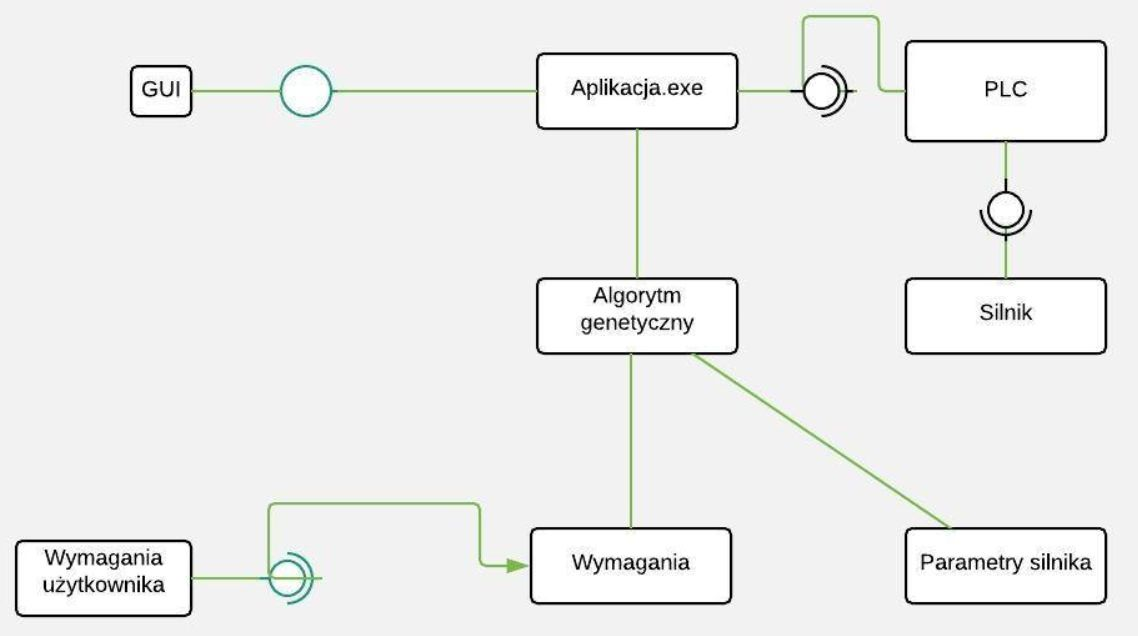
\includegraphics[scale=0.5]{komponent}
\caption{Struktura systemu i wyszczególnienie jego komponentów składowych}
\label{komponent}
\end{figure} 
\newpage
\begin{figure}[h!]
\centering
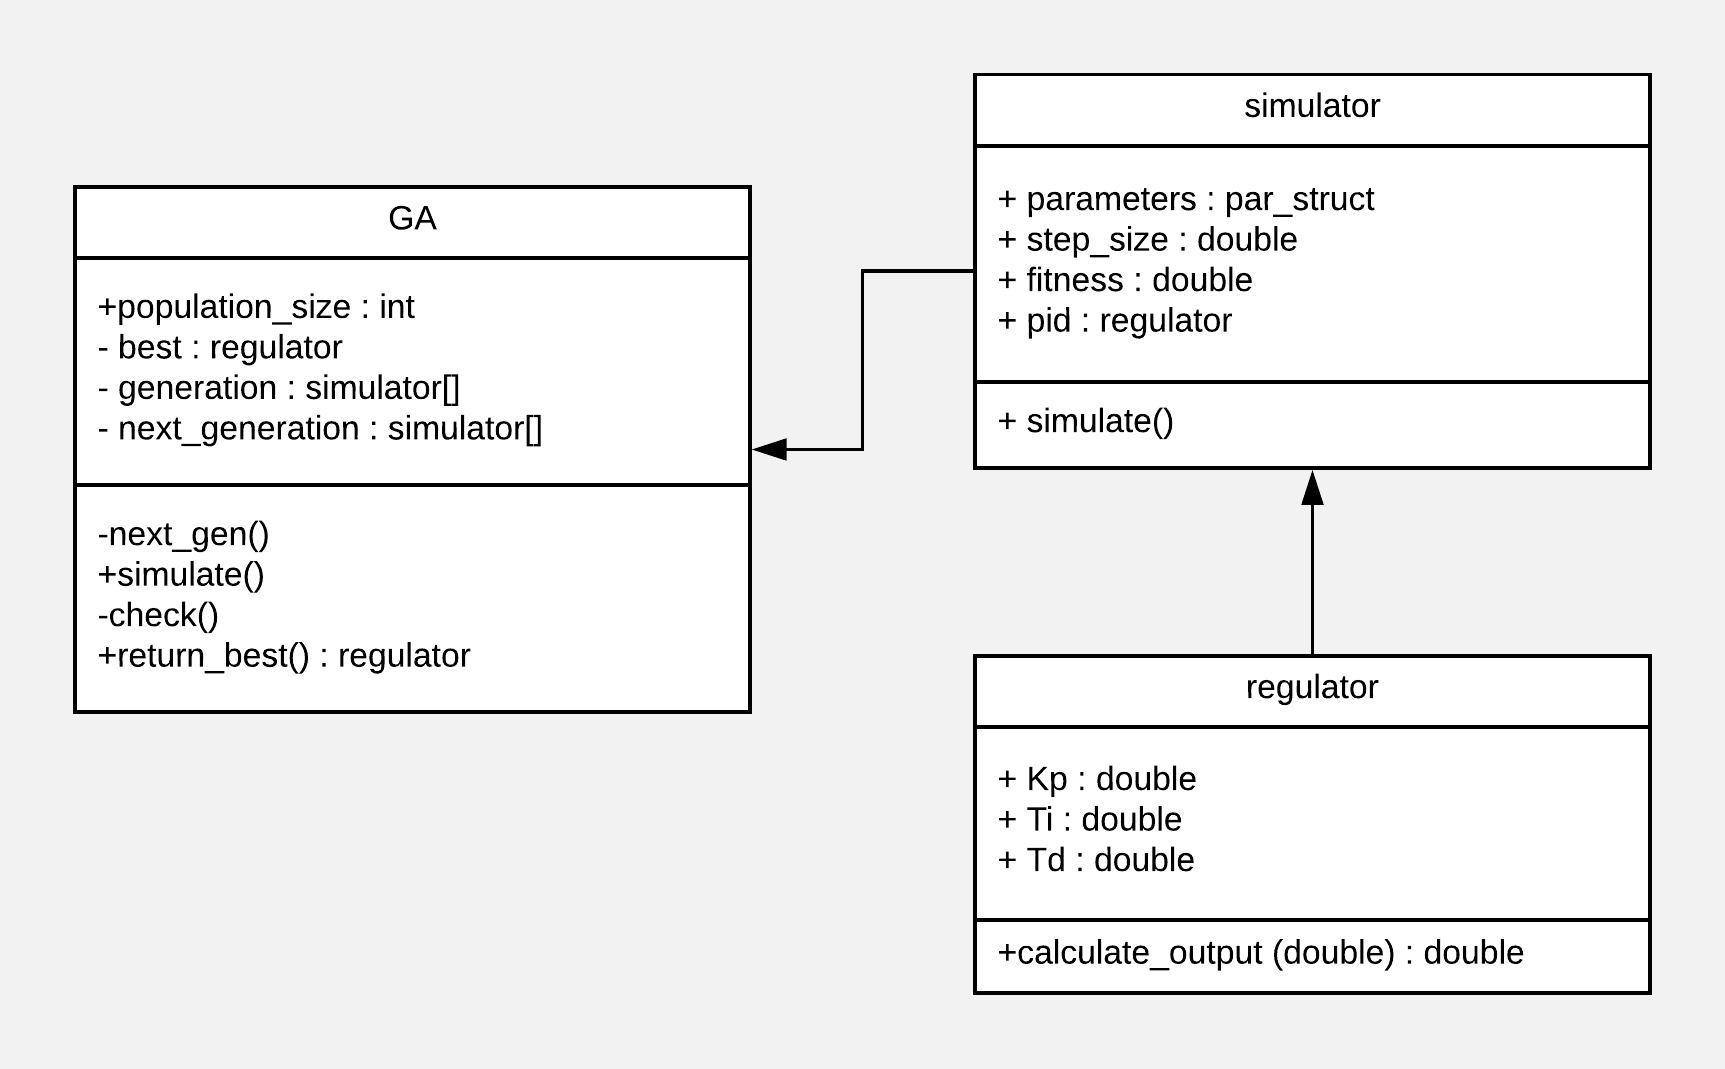
\includegraphics[scale=0.25]{klasa}
\caption{Diagram przedstawiający strukturę klas w oprogramowaniu systemu}
\label{klasa}
\end{figure}
Na rysunkach \ref{komponent} oraz \ref{klasa} przedstawiono wyszczególnione komponenty całego systemu oraz klasy składowe jego oprogramowania.\
\subsection{Scenariusze użycia systemu}
\indent Przykładowy, zakładany scenariusz użycia systemu ukazujący interakcję pomiędzy jego poszczególnymi komponentami podczas realizacji określonych zadań, przedstawiony został na rysunku \ref{aktywnosc}, znajdującym się na następnej stronie.\newpage
\begin{figure}[ht!]
\centering
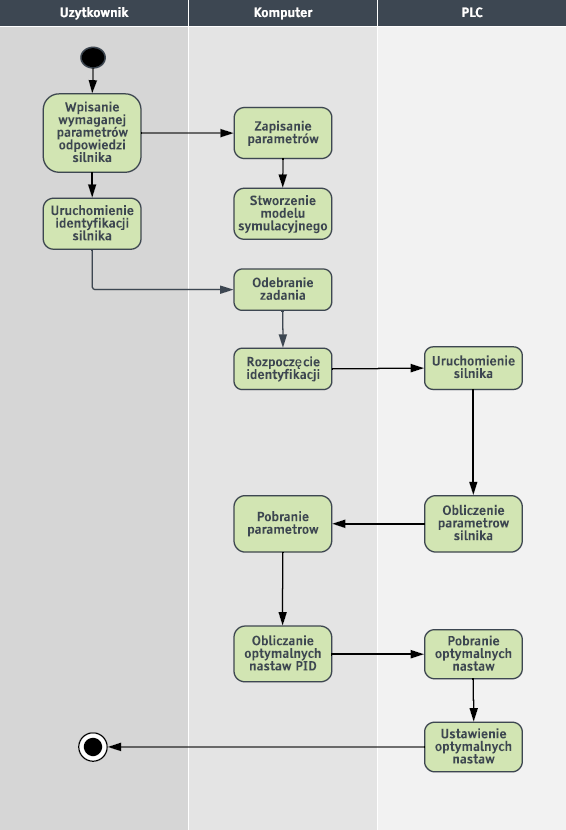
\includegraphics[scale=1]{aktywnosc}
\caption{Diagram aktywności dla omawianego systemu}
\label{aktywnosc}
\end{figure}

\newpage

%% DRUGA CZESC - DOKUMENTACJA TECHNICZNA %%

\section{Specyfikacja techniczna}
\indent Główna aplikacja opracowana zostanie przy użyciu środowiska Microsoft Visual Studio. Do implementacji głównej aplikacji zawierającej zaimplementowany algorytm genetyczny i interfejs użytkownika wykorzystane zostaną podstawowe biblioteki standardowe dostępne w środowisku Visual Studio. \newline
\indent Narzędziem dodatkowo wspomagającym opracowywanie oprogramowania systemu jest system kontroli wersji GIT - GitHub. \newline
\indent Sterownik PLC wykorzystywany do zrealizowania omawianego systemu to moduł S7-1200 firmy Siemens. Komunikacja pomiędzy stacją operatorską (PC, tablet, laptop) a sterownikiem PLC realizowana będzie przy użyciu sieci Ethernet.\newline
\indent Kluczowe elementy omawianego systemu przedstawiono na wcześniej zamieszczonych diagramach UML.Poniżej umieszczono diagram UML ukazujący interakcje pomiędzy składowymi elementami oprogramowania.
\begin{figure}[ht!]
\centering
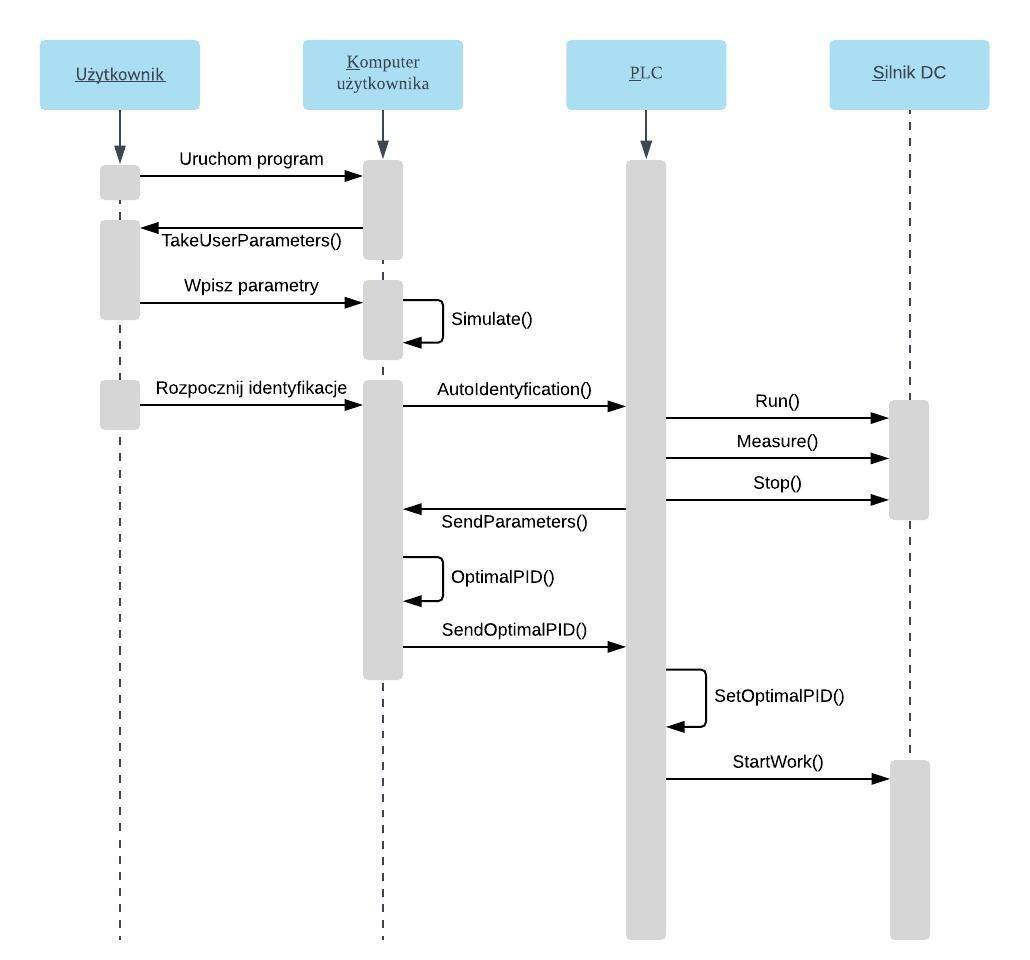
\includegraphics[scale=0.42]{uml}
\caption{Diagram UML przedstawiający interakcje pomiędzy składowymi oprogramowania i systemu}
\label{komponent2}
\end{figure} 
\newpage
\subsection{Harmonogram i podział pracy}
\begin{table}[ht]
	  \caption{Harmonogram prac związanych z realizacją projektu}
    \begin{tabular}{|c|c|l|}
    \hline
    \multicolumn{1}{|c|}{Lp.} & \multicolumn{1}{c|}{Data zakończenia zadań} & \multicolumn{1}{c|}{Zadania do zrealizowania} \\
    \hline
       1.  &16.05.2018 & \begin{tabular}{  L{0.55\textwidth}  m{0.45\textwidth} | }1. Określenie użytkowników końcowych systemu, na podstawie rozmów z klientem.\\2. Zdefiniowanie wymagań funkcjonalnych i pozafunkcjonalnych dla opracowywanego systemu.\\3. Opracowanie dokumentacji funkcjonalnej, zawierającej powyższe informacje oraz scenariusz użycia systemu i odpowiednie diagramy UML. \\ 4. Prezentacja aktualnych efektów prac nad projektem przed docelowym klientem.\end{tabular} \\
    \hline
       2.  &23.05.2018 & \begin{tabular}{  L{0.55\textwidth}  m{0.45\textwidth} | } 1. Utworzenie oraz odpowiednia organizacja repozytorium projektu w serwisie GitHub.com.\\ 2. Wybór języka programowania, środowiska IDE, bibliotek zastosowanych do opracowania oprogramowania.\\ 3. Opracowanie specyfikacji technicznej zawierającej m.in. modele UML kluczowych elementów systemu. \\ 4. Prezentacja aktualnych efektów prac nad projektem przed docelowym klientem. \\ \end{tabular} \\
    \hline
       3.  &06.06.2018  &  \begin{tabular}{  L{0.55\textwidth}  m{0.45\textwidth} | } 1. Opracowanie modelu matematycznego silnika DC. \\
       2. Rozpoczęcie opracowywania oprogramowania aplikacji i jej interfejsu graficznego.\\ 3. Rozpoczęcie implementacji optymalizatora nastaw i komunikacji z PLC. \\ 4. Opracowanie dokumentacji wykonanych prac. 5. Konsultacja otrzymanych wyników prac z docelowym klientem. \\ \end{tabular} \\
    \hline
       4.  & 13.06.2018      & \begin{tabular}{  L{0.55\textwidth}  m{0.45\textwidth} | } 1. Wykonanie odpowiednich cykli testów jednostkowych oprogramowania. \\2. Profilowanie aplikacji i próba optymalizacji hot spotów.\\ 3. Odpowiednie udokumentowanie przebiegu wykonywanych testów.\\ 4. Przedstawienie klientowi dotychczasowych wyników i wykonanie ewentualnych poprawek.\\ \end{tabular} \\
    \hline
       5.  & 30.06.2018     & \begin{tabular}{  L{0.55\textwidth}  m{0.45\textwidth} | } 1. Implementacja aplikacji na rzeczywistym obiekcie.\\ 2. Wykonanie serii testów działania systemu w warunkach docelowych. \\ 3. Naniesienie poprawek do oprogramowania systemu i ich dokumentacja.\\4. Oddanie systemu do użytku klienta.\\ \end{tabular} \\
    \hline
    \end{tabular}
  \label{tabelka}
\end{table}
\indent Realizacja omawianego systemu, którego charakterystykę i opis przedstawiono w niniejszym opracowaniu wymaga odpowiedniego zaplanowania prac zespołu, które umożliwią zakończenie całego projektu sukcesem. Harmonogram prac związanych z opracowaniem oprogramowania i realizacją całości systemu przedstawiono w tabeli \ref{tabelka} znajdującej się na następnej stronie.
	


\indent Na podstawie zdefiniowanych wymagań dotyczących funkcjonalności systemu zdefiniowano następujący podział pracy w zespole:
\vspace{0.3cm}
\begin{itemize}
\item \textbf{Kamil Andrzejewski} - prowadzenie porządku w repozytorium - GIT maintainer, komunikacja PLC
\item \textbf{Maciej Zielonka} - implementacja algorytmu genetycznego, implementacja aplikacji optymalizującej
\item \textbf{Paweł Zarembski} - zaprojektowanie i implementacja interfejsu użytkownika
\item \textbf{Paweł Spławski} - tworzenie dokumentacji projektu, opracowanie modelu silnika DC
\end{itemize}


%% KOLEJNA CZESC DOKUMENTACJI %%



\renewcommand{\baselinestretch}{1.5}\normalsize	% powrót do interlinii 1.5 na wypadek dodatków
\end{document}	% musi być na samiutkim końcu
\grid
